\documentclass[../main.tex]{subfiles}

\begin{document}
\section{Results}\label{sec:results}

Here we present figures showing the results of the simulations we have produced of the solar system. 

\subsection{Earth-Sun}

\begin{figure}[htb!]
    \centering
    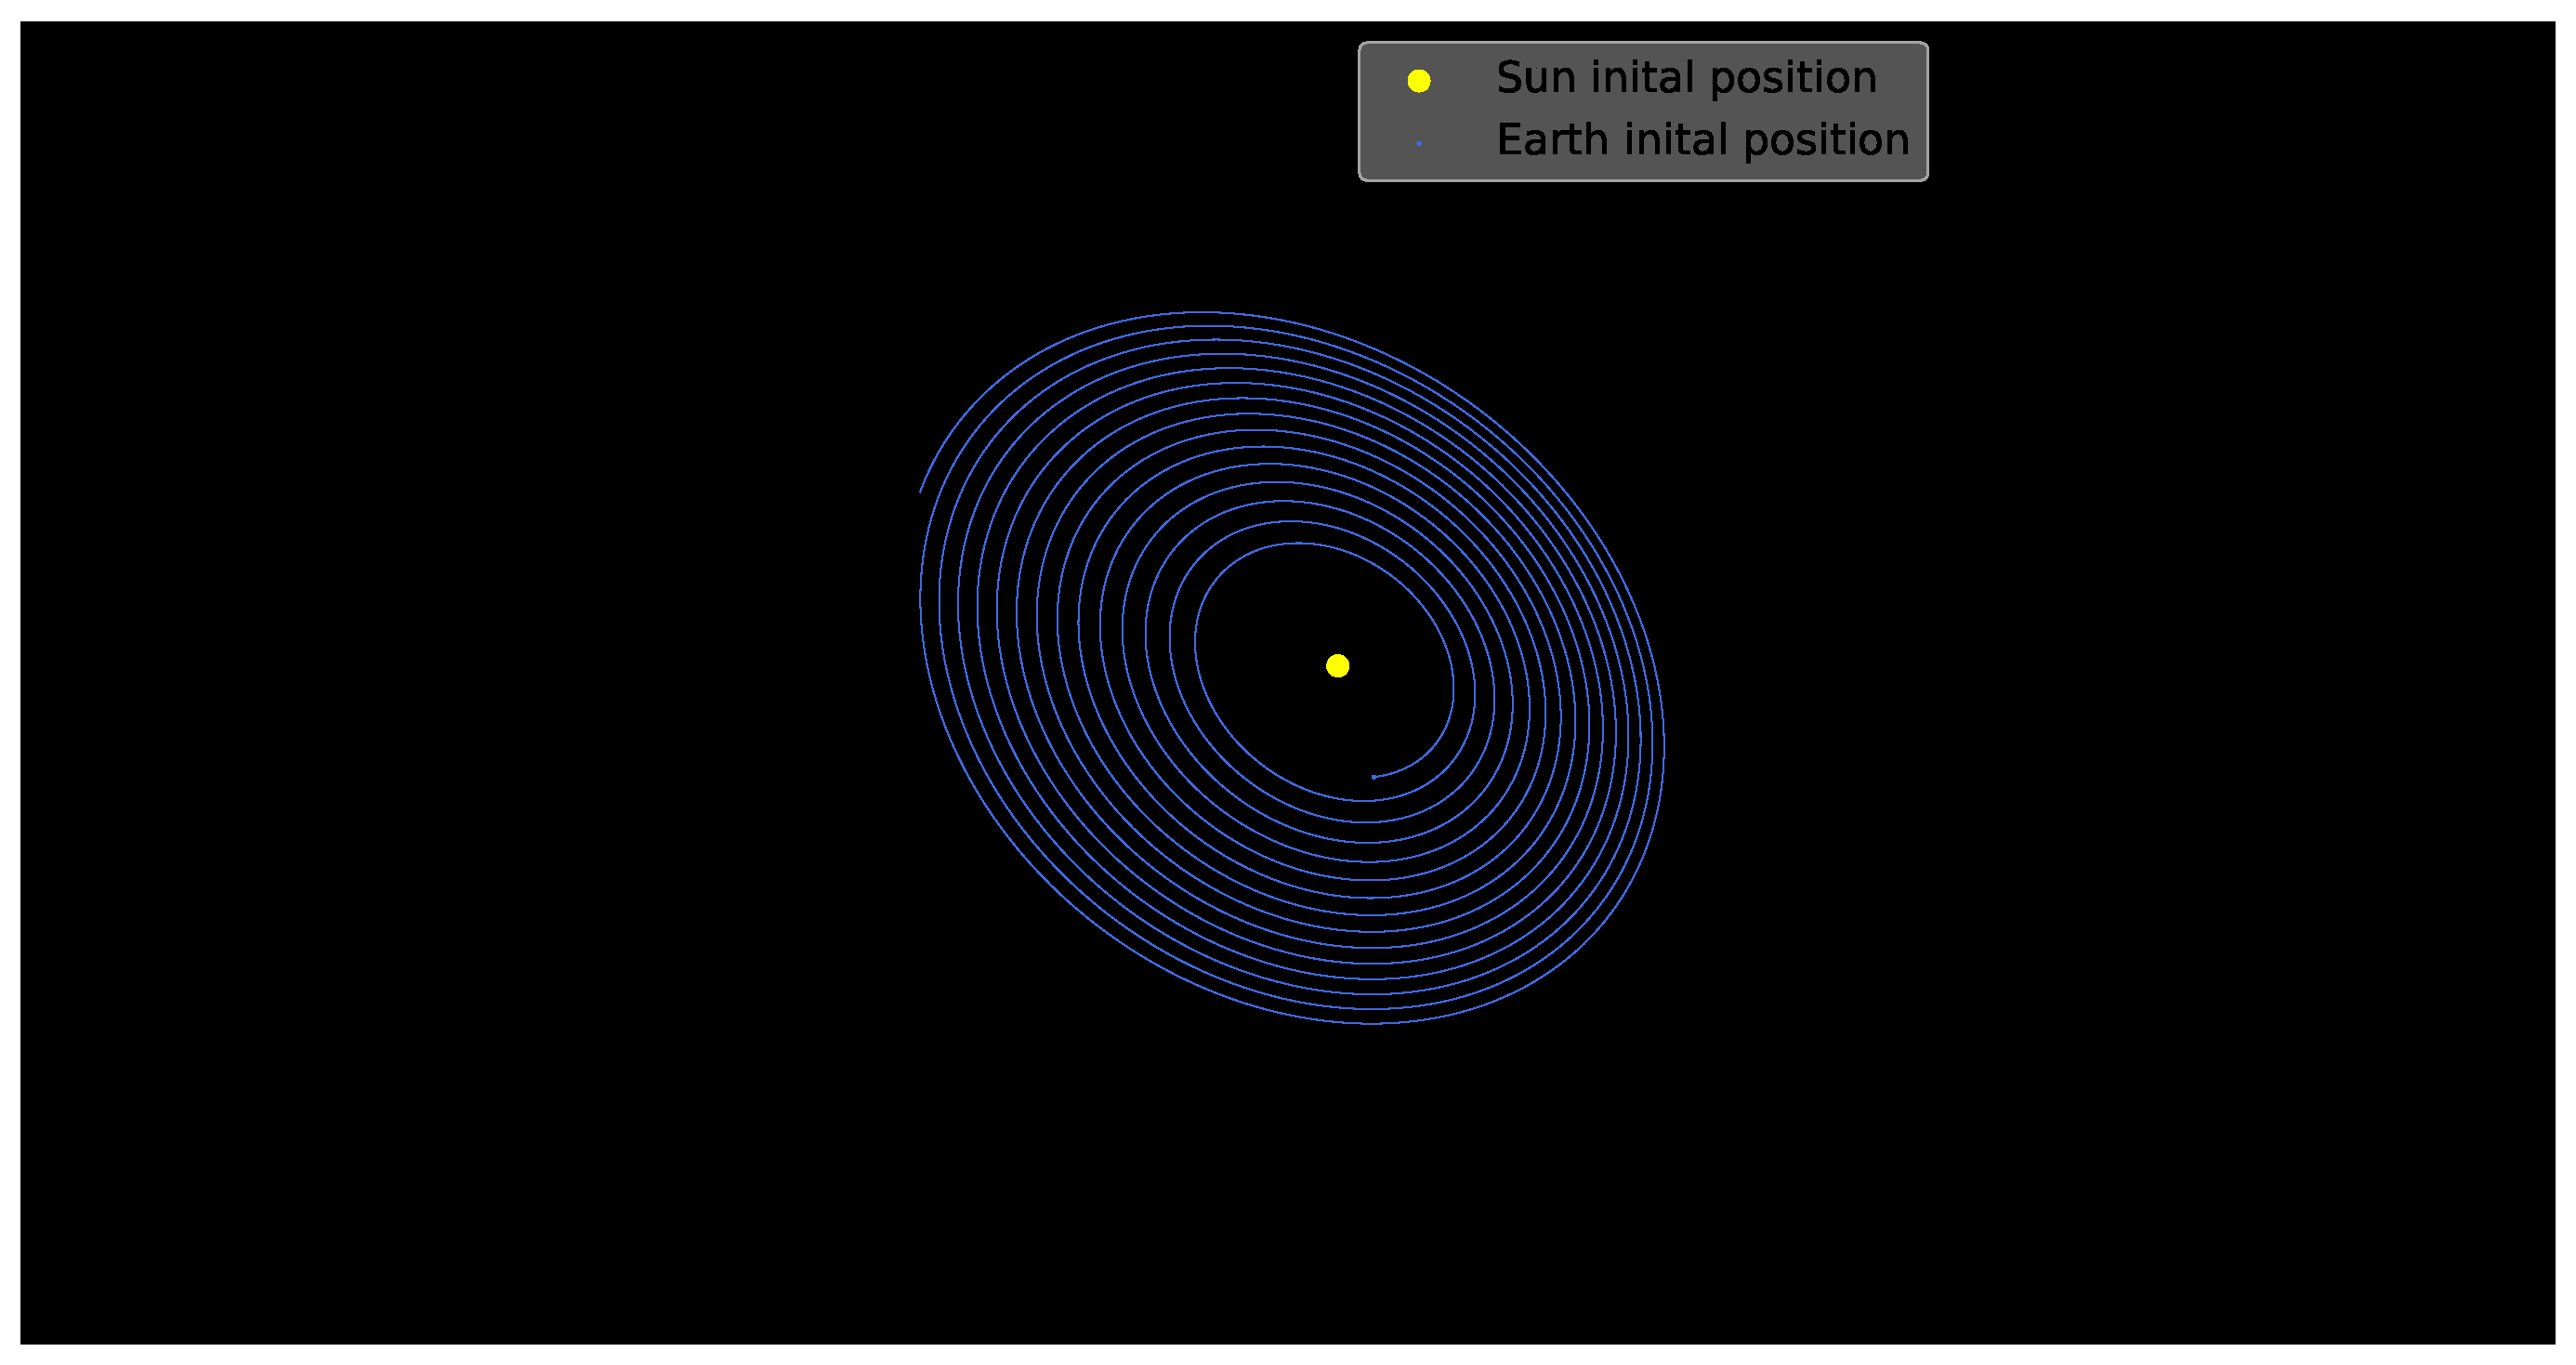
\includegraphics[trim=15cm 5.cm 11cm 0.cm, clip,width=0.8\textwidth]{../figures/Euler_Earth_Sun.pdf}
    \caption{Here is the Earth-Sun system simulated over 50 years using the Euler method. The Earth does not form a closed orbit, and is slowly escaping the gravitational well of the Sun. This is an error caused by the fact that the Euler method does not conserve energy.}
    \label{fig:earth-sun-euler}
\end{figure}

\begin{figure}[htb!]
    \centering
    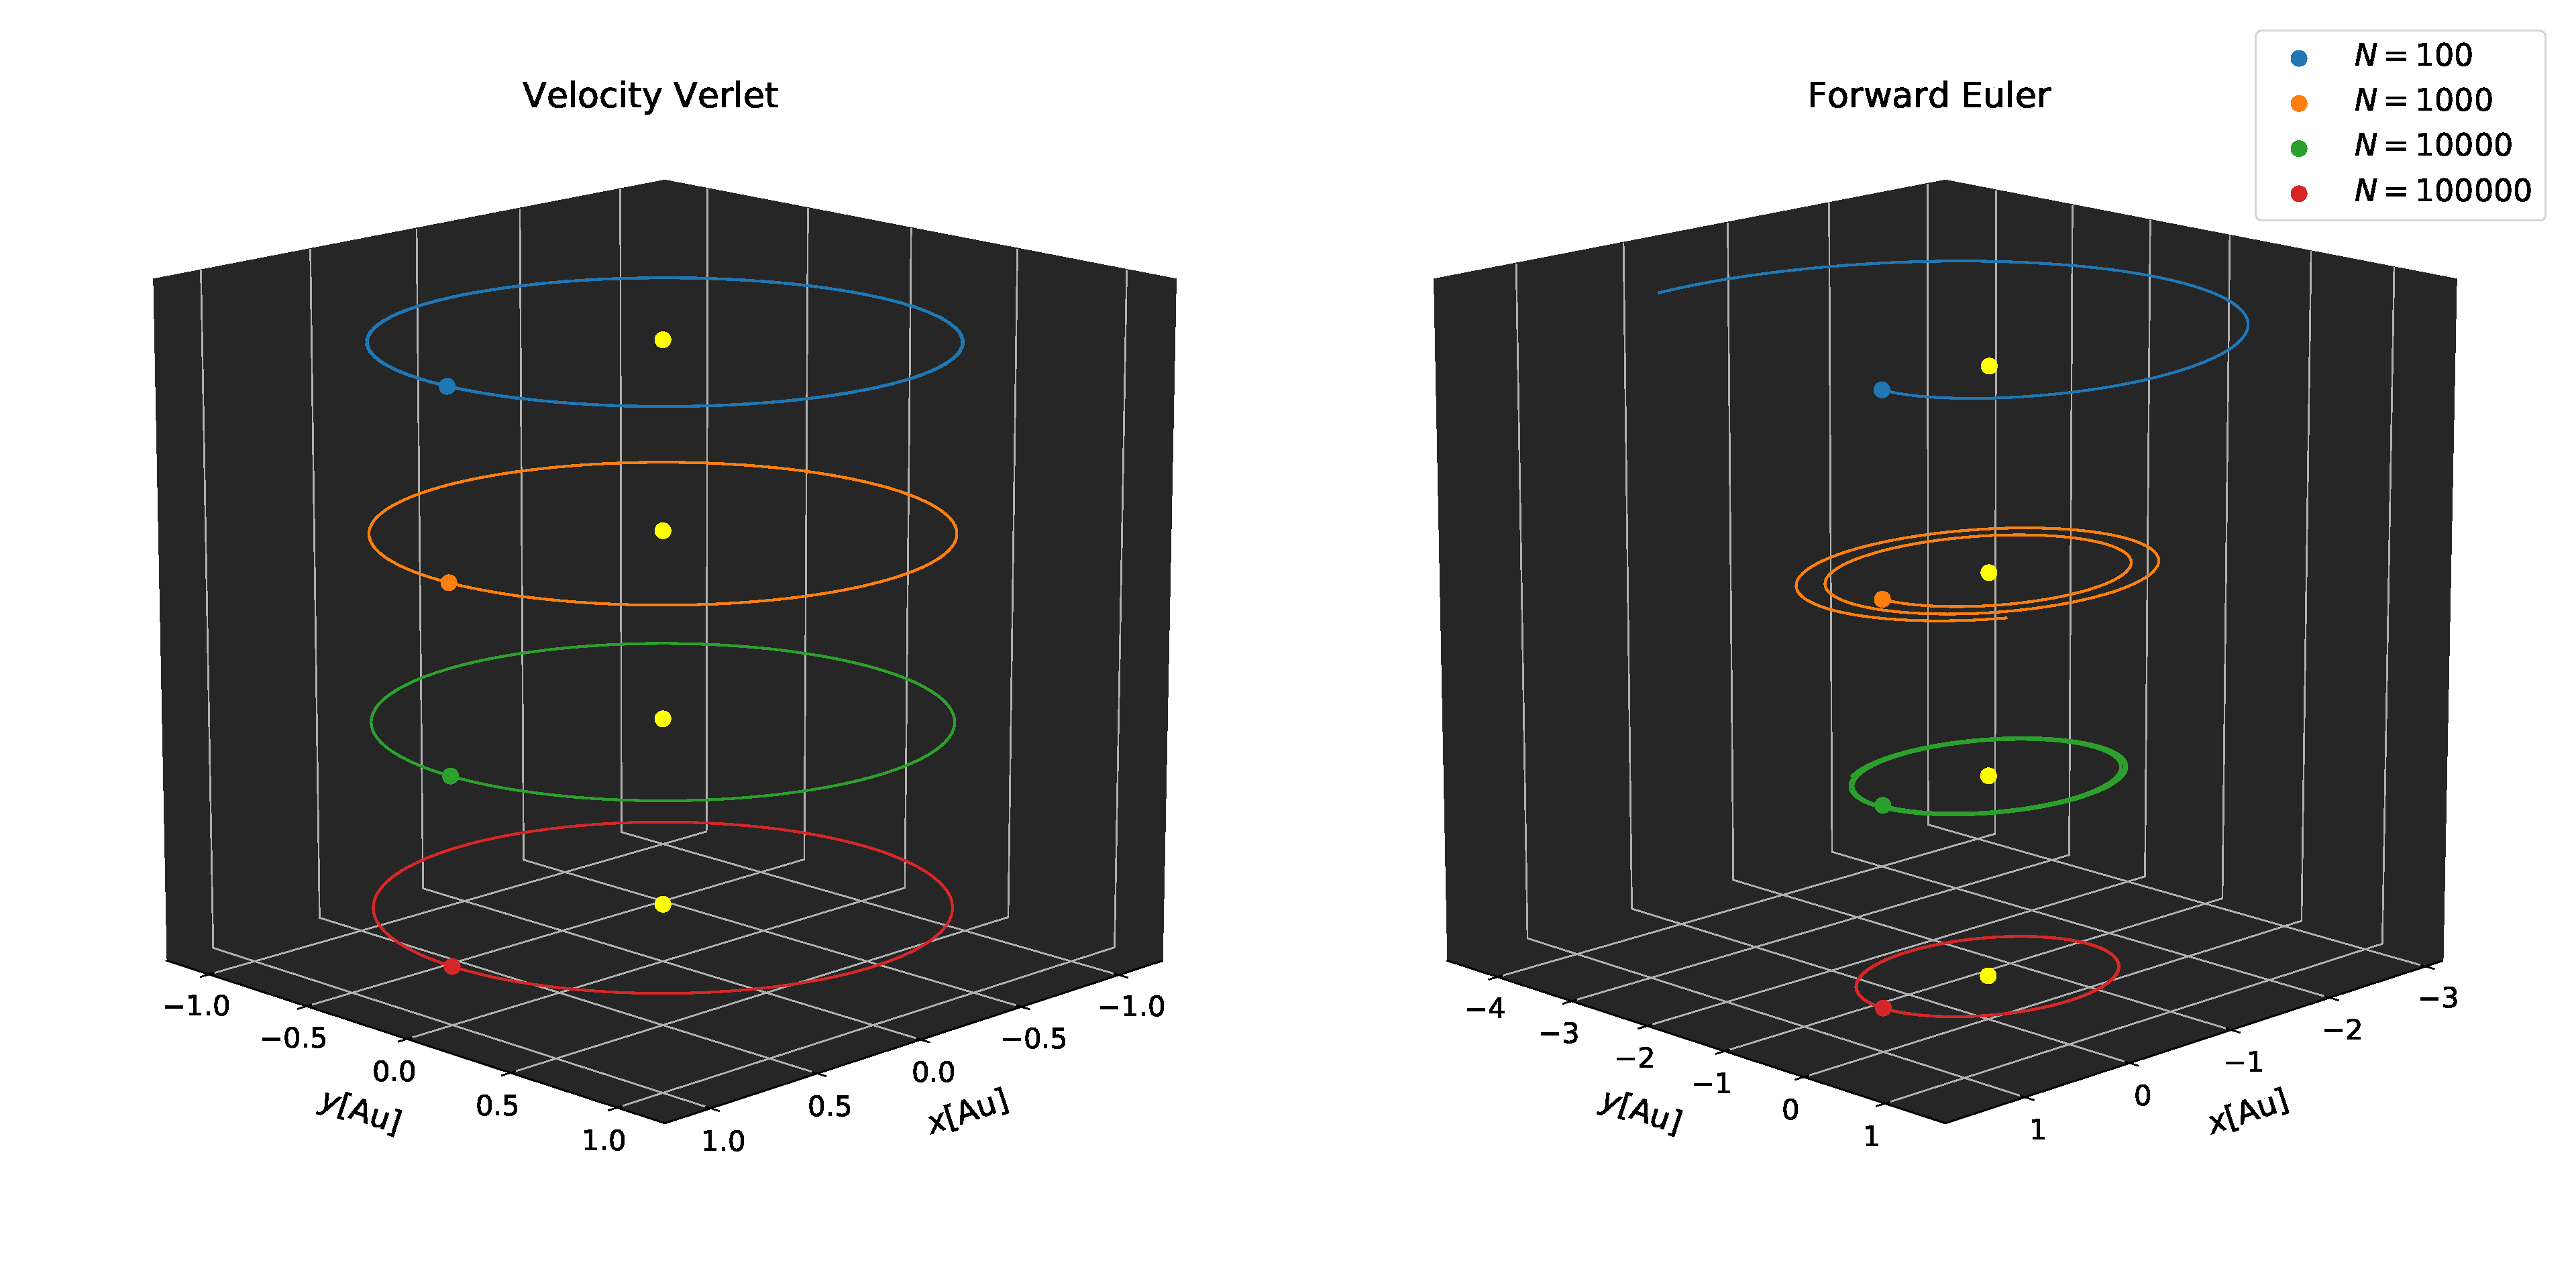
\includegraphics[trim=2cm 0.cm 2cm 0.cm, clip,width=\textwidth]{../figures/stability.pdf}
    \caption{}
    \label{fig:earth-sun-verlet-vs-euler}
\end{figure}

\subsection{Escape Velocity}

To find the escape velocity of the Earth in the Earth-Sun system numerically, simple trial and error was used. The results are shown in \cref{fig:earth-escape-velocity}, and the final value of the initial velocity $v_0$ that was sufficient for the earth to leave the solar system is $v_0 = 2.4296 \cdot 10^{-2} \frac{\text{AU}}{\text{day}}$.

\begin{figure}[htb!]
    \centering
    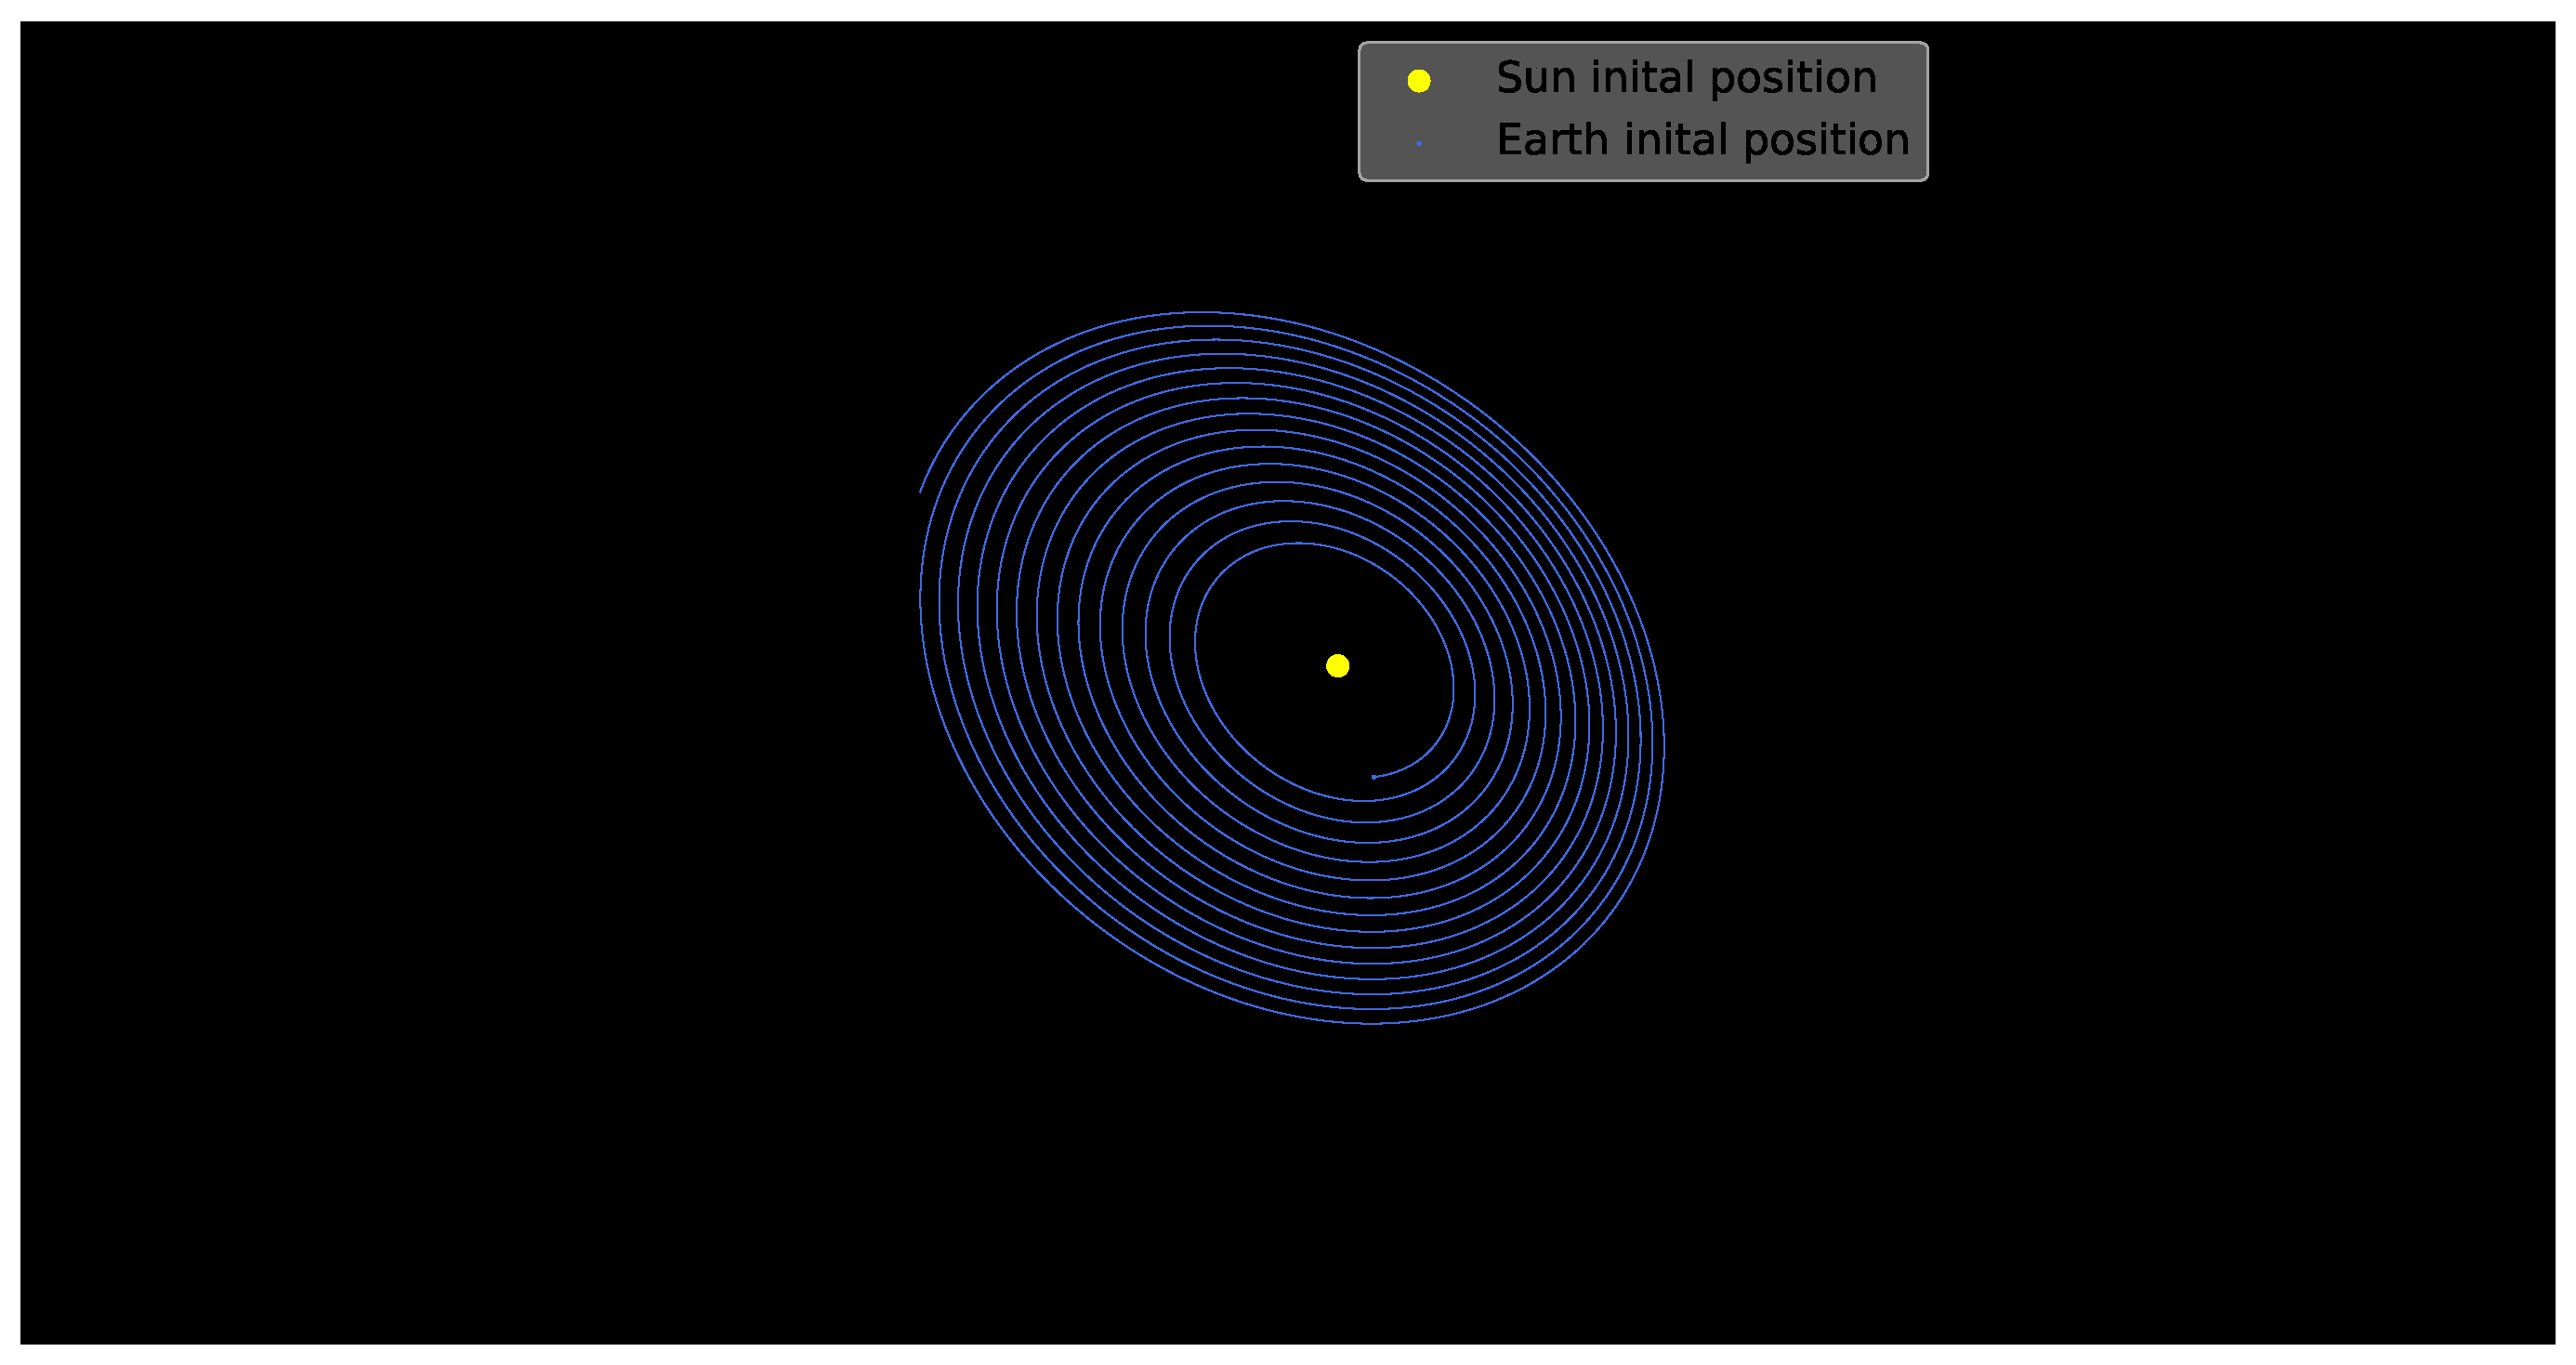
\includegraphics[trim=15cm 5.cm 11cm 0.cm, clip,width=0.8\textwidth]{../figures/Euler_Earth_Sun.pdf}
    \caption{Pictured is a simulation over 248 years, with the initial velocity of the earth set to $v_0 = 2.4296 \cdot 10^{-2} \frac{\text{AU}}{\text{day}}$. By trial and error, this value seems to be enough for }
    \label{fig:earth-escape-velocity}
\end{figure}

Figure of the Earth escaping the sun's gravitational field. Seems that the presence of the remaining planets does little to change the escape velocity. Preliminary results suggests that escape velocity is about 2.42E-02 AU/day, corresponding with the approximate 2.433E-02 AU/day analytic answer.

\subsection{Three-body Problem}
We have implemented a model consisting of the Sun, Earth and Jupiter, employing the velocity Verlet method. \Cref{fig:three-body-problem} shows the simulated orbits of the celestial bodies in our model for 10 years. The top subfigure shows the simulation with Jupiter's usual mass, $M_j$. We also model the scenarios where Jupiter's mass is $10M_j$ and $1000M_j$, which is shown in the middle and bottom subfigure, respectively. As one can see from \cref{fig:three-body-problem}, a mass of $10M_j$ would drag the Earth closer to the Sun, while a mass of $1000M_j$ would pull the entire system apart. 

\begin{figure}[htb!]
    \centering
    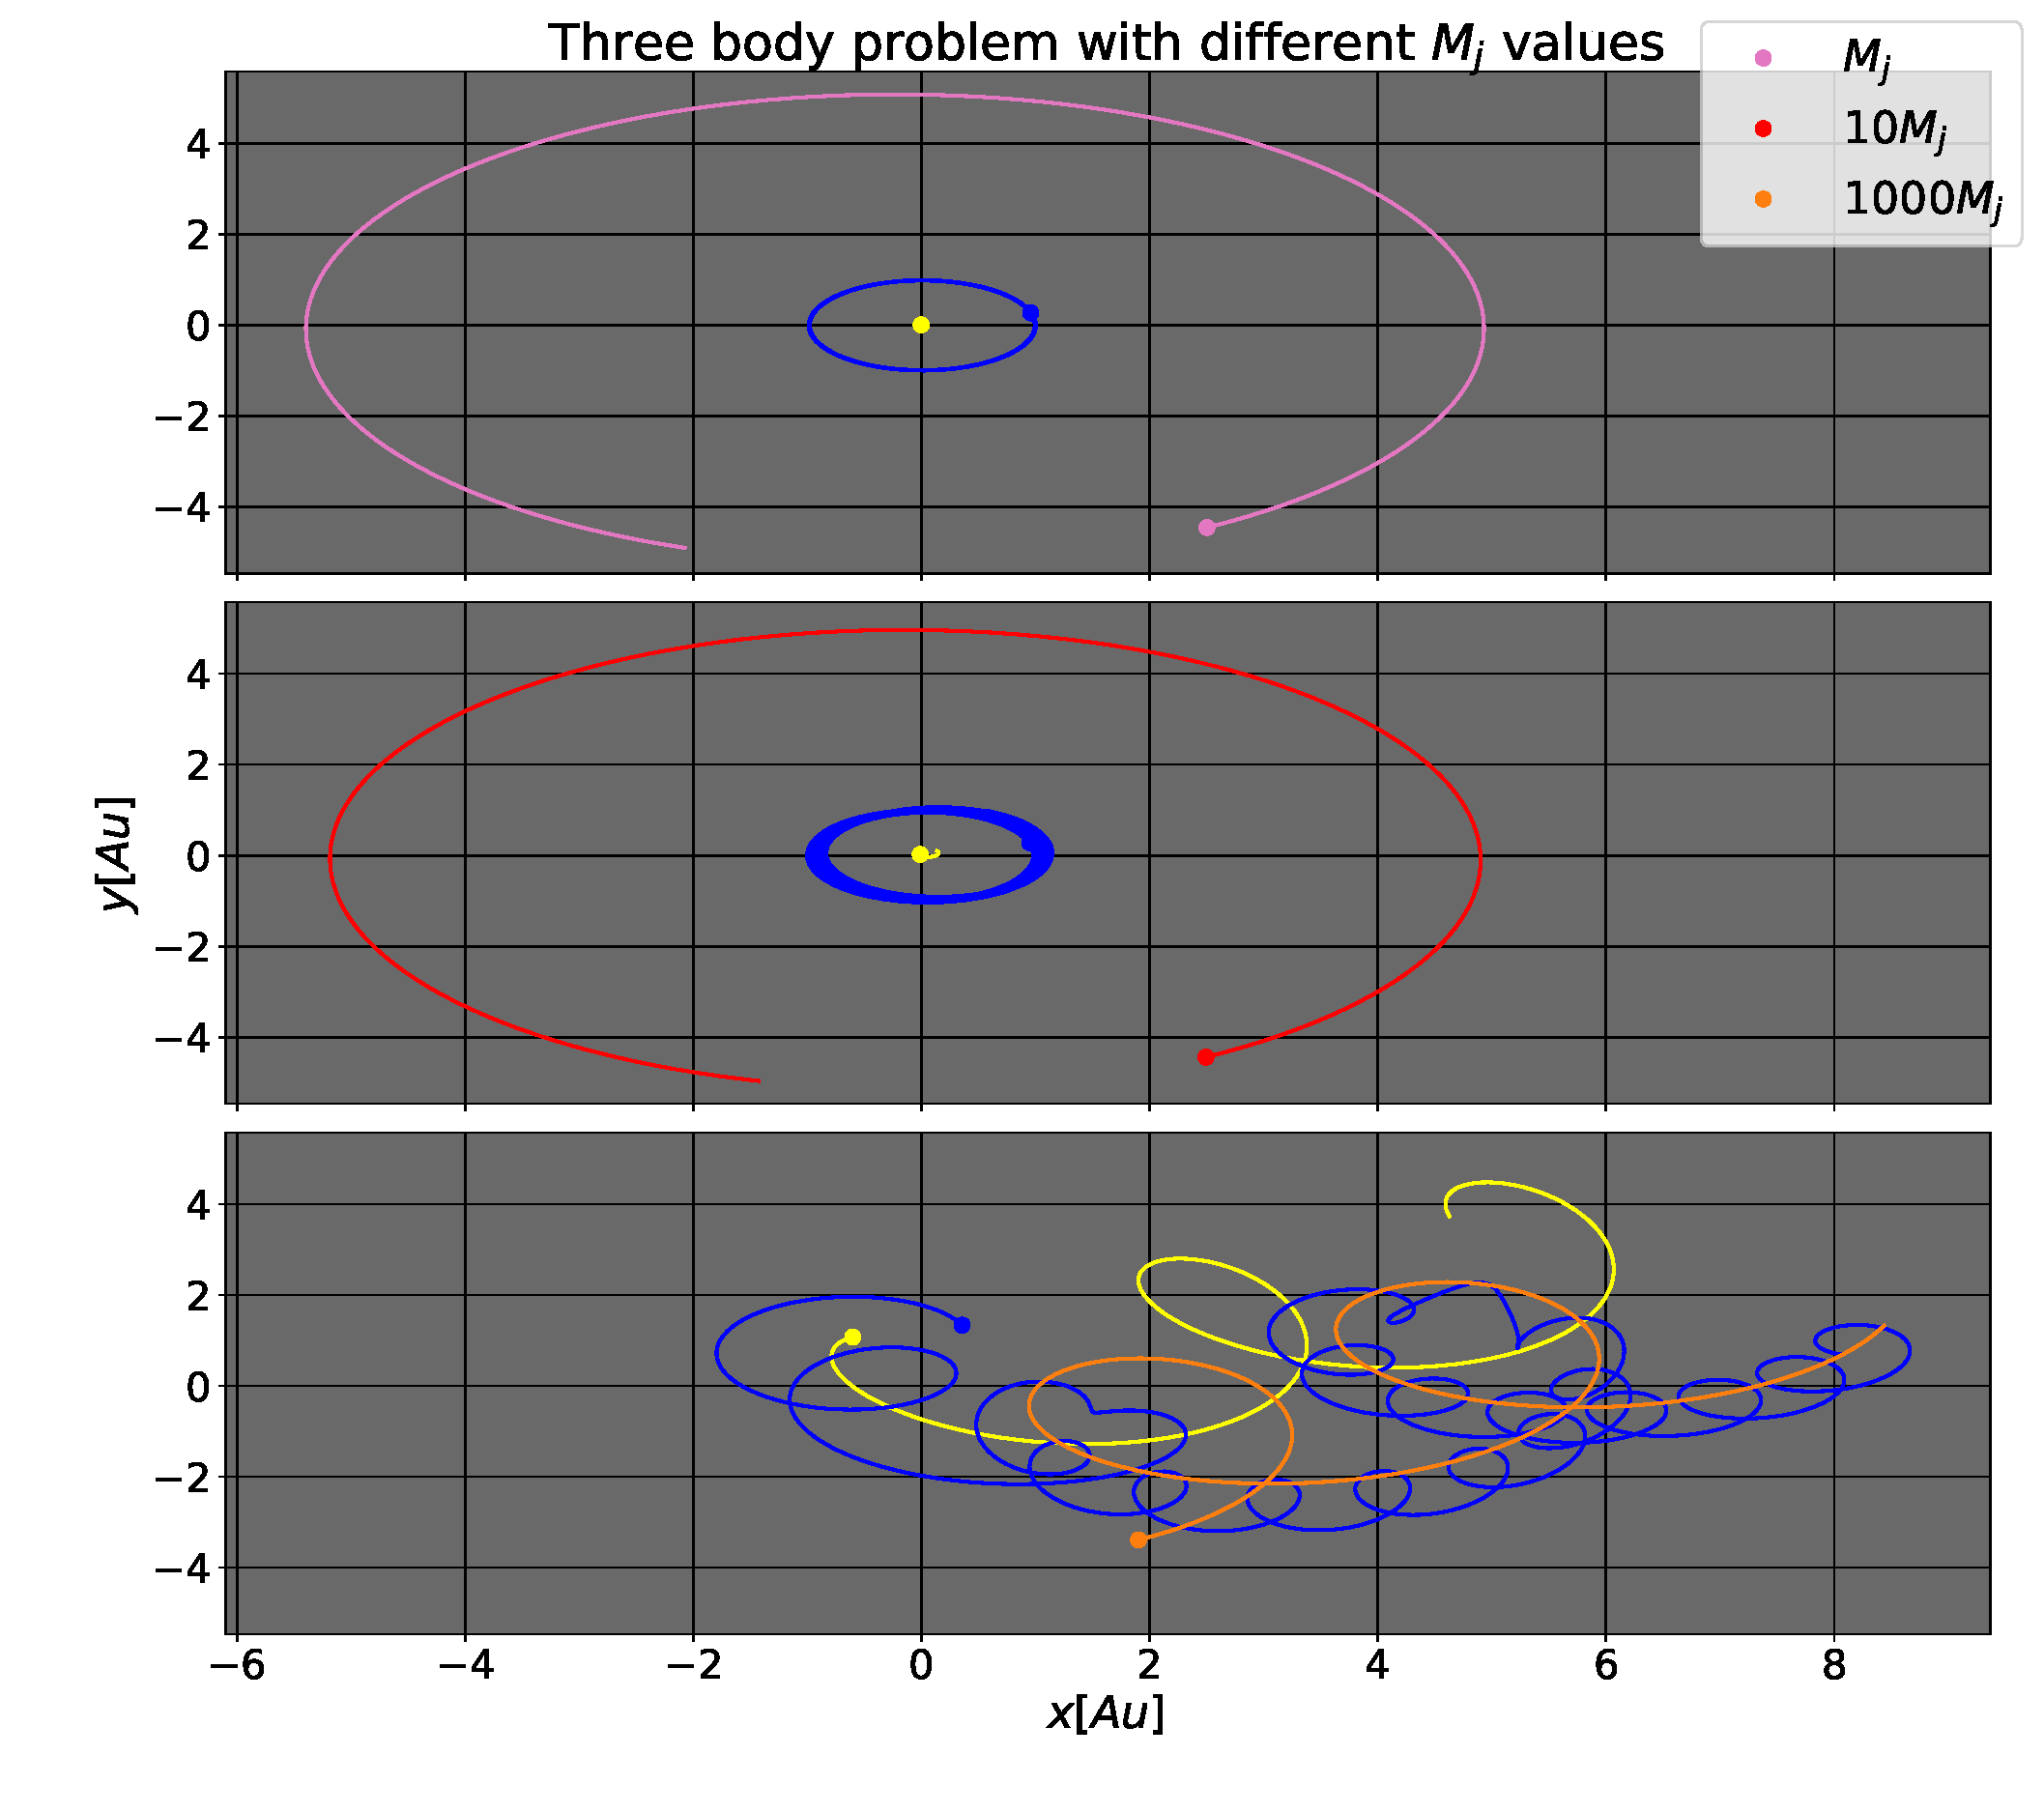
\includegraphics[width=0.9\textwidth]{../figures/three_body_problem.pdf}
    \caption{Plot of the simulated orbit of the Sun, Earth and Jupiter system for 10 years with: \textbf{top:} Jupiter's usual mass, $M_j$, \textbf{middle:} $10M_j$ \textbf{bottom:} $1000M_j$}.
    \label{fig:three-body-problem}
\end{figure}


\subsection{Perihelion Precession}

Applying the relativistic correction in \cref{eq:rel-correction} to the classical Newtonian equation of gravity, we simulated one century of only Mercury and the Sun. Starting at perihelion, the point closest to the Sun, we simulated with relativistic corrected gravity and without. The angles between the coordinates of the first perihelion and the coordinates of subsequent perihelions are plotted in \cref{fig:perihelion-precession}, against the observed $43''$ precession per century.

\begin{figure}[htb!]
    \centering
    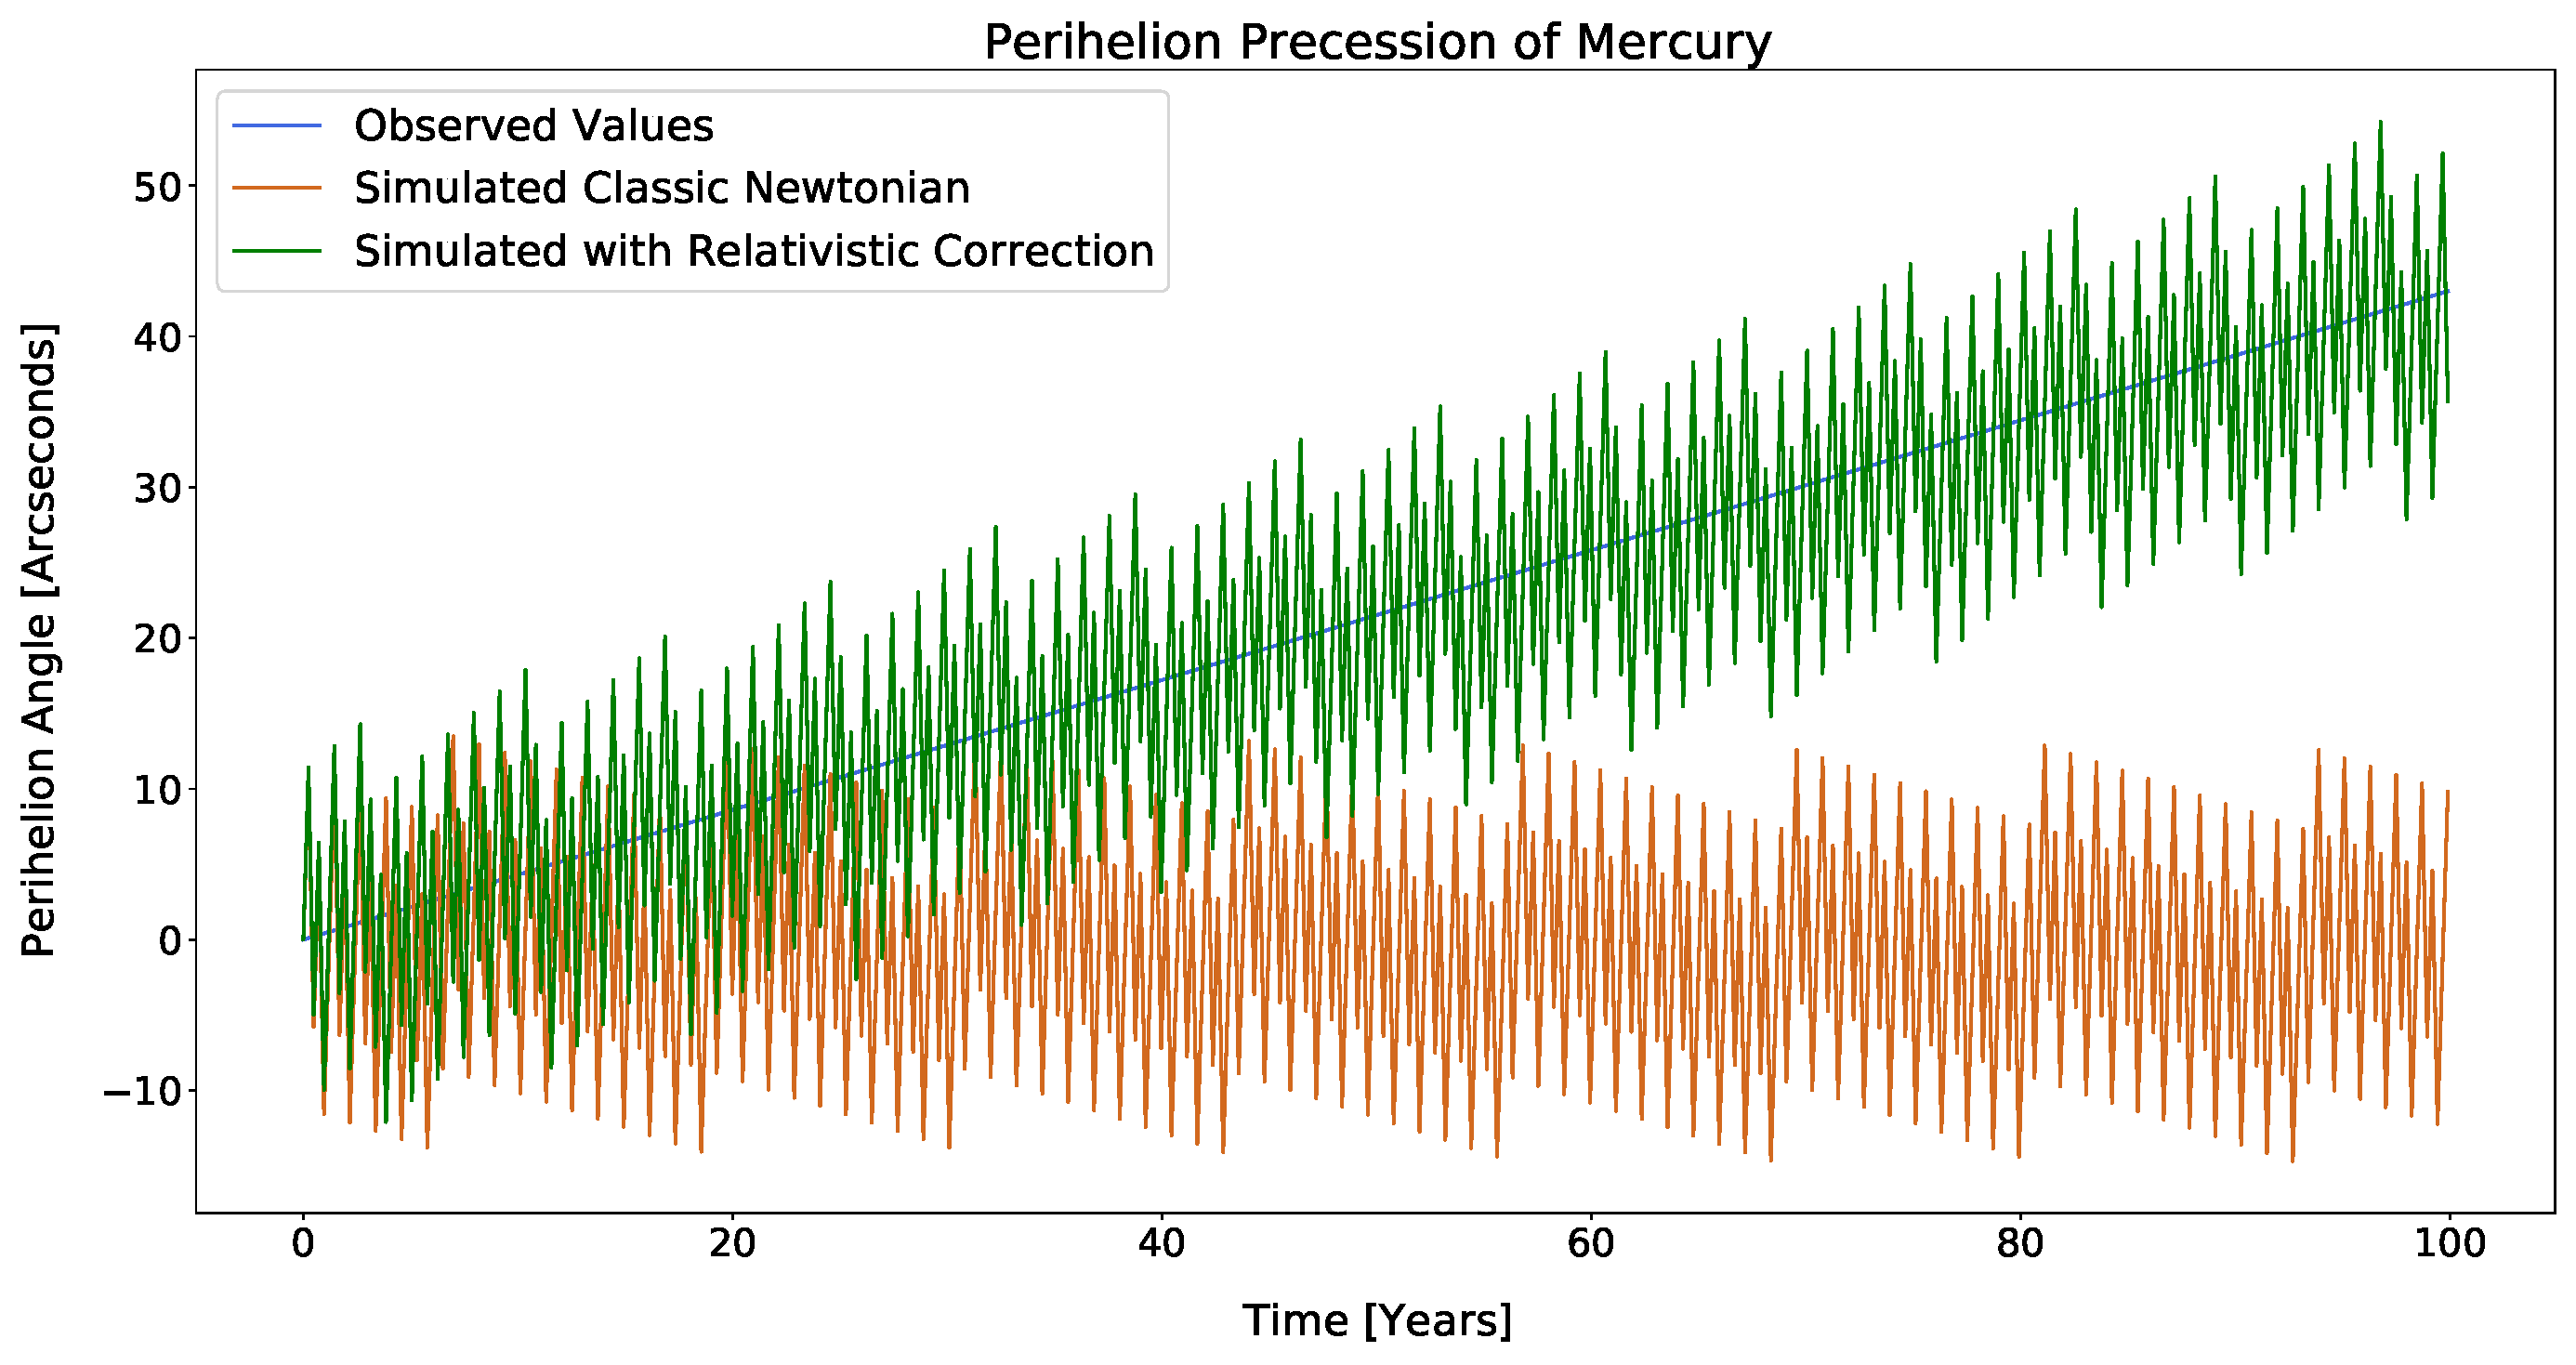
\includegraphics[width=1.0\textwidth]{../figures/3-10^7 perihelion.pdf}
    \caption{Plot of the perihelion angle of Mercury as a function of time, for observed and simulated values, with and without relativistic correction. While the simulated data is noisy, it is clear that the relativistic correction follows the observed values closely.}
    \label{fig:perihelion-precession}
\end{figure}

\end{document}
